% This LaTeX was auto-generated from MATLAB code.
% To make changes, update the MATLAB code and export to LaTeX again.

\documentclass{article}

\usepackage[utf8]{inputenc}
\usepackage[T1]{fontenc}
\usepackage{lmodern}
\usepackage{graphicx}
\usepackage{color}
\usepackage{listings}
\usepackage{hyperref}
\usepackage{amsmath}
\usepackage{amsfonts}
\usepackage{epstopdf}
\usepackage[table]{xcolor}
\usepackage{matlab}

\sloppy
\epstopdfsetup{outdir=./}
\graphicspath{ {./sndtestInteractive_images/} }

\matlabmultipletitles

\begin{document}

\begin{matlabcode}
clear;
% Author: Gustav Kjellberg

\end{matlabcode}

\matlabtitle{Lab 2 - Feature extraction}


\vspace{1em}

\matlabheadingthree{First, let's read the data from the three different tracks.}

\begin{par}
\hfill \break
\end{par}

\begin{matlabcode}
[Y1, FS1] = audioread('Songs/melody_1.wav');
[Y2, FS2] = audioread('Songs/melody_2.wav');
[Y3, FS3] = audioread('Songs/melody_3.wav');

\end{matlabcode}


\matlabheadingthree{Then, set the length of the window, 0.03 is default.}

\begin{par}
\hfill \break
\end{par}

\begin{matlabcode}

lengthOfWindow = 0.03
\end{matlabcode}
\begin{matlaboutput}
lengthOfWindow = 0.0300
\end{matlaboutput}
\begin{matlabcode}

\end{matlabcode}


\matlabheadingthree{Use the data yielded from audioread and extract the 3 features}

\begin{itemize}
\setlength{\itemsep}{-1ex}
   \item{\begin{flushleft} Pitch: frIseq(1,:) 80 - 1100 Hz \end{flushleft}}
   \item{\begin{flushleft} Correlation coefficient ($\rho$): frIseq(2,:)  \end{flushleft}}
   \item{\begin{flushleft} Esitmates of per-sample intensity: frIseq(3,:) \end{flushleft}}
\end{itemize}

\begin{matlabcode}
frIseqT1 = GetMusicFeatures(Y1,FS1,lengthOfWindow);
frIseqT2 = GetMusicFeatures(Y2,FS2,lengthOfWindow);
frIseqT3 = GetMusicFeatures(Y3,FS3,lengthOfWindow);

\end{matlabcode}


\begin{matlabcode}

\end{matlabcode}


\matlabheadingthree{Plot the frequencies for the three different signals. Note that two melodies are from the same song and should thus be similair.}

\begin{par}
\hfill \break
\end{par}

\begin{matlabcode}

figure;
sgtitle('Pitch of melodies as a function of time');
fig1 = subplot(3,1,1);
t_1 = 0.00:lengthOfWindow:(length(frIseqT1(1,:))-1)*0.03;
plot(t_1, frIseqT1(1,:));
xlabel('Time (S)');
ylabel('Pitch (Hz)');
title('Melody_1')

fig2 = subplot(3,1,2);
t_2 = 0.00:lengthOfWindow:(length(frIseqT2(1,:))-1)*0.03;
plot(t_2, frIseqT2(1,:));
xlabel('Time (S)');
ylabel('Pitch (Hz)');
title('Melody_2')

fig3 = subplot(3,1,3);
t_3 = 0.00:lengthOfWindow:(length(frIseqT3(1,:))-1)*0.03;
plot(t_3, frIseqT3(1,:));
xlabel('Time (S)');
ylabel('Pitch (Hz)');
title('Melody_3')
set([fig1 fig2 fig3], 'YScale','log');
set([fig1 fig2 fig3], 'YLim', [100 300]);
\end{matlabcode}
\begin{center}
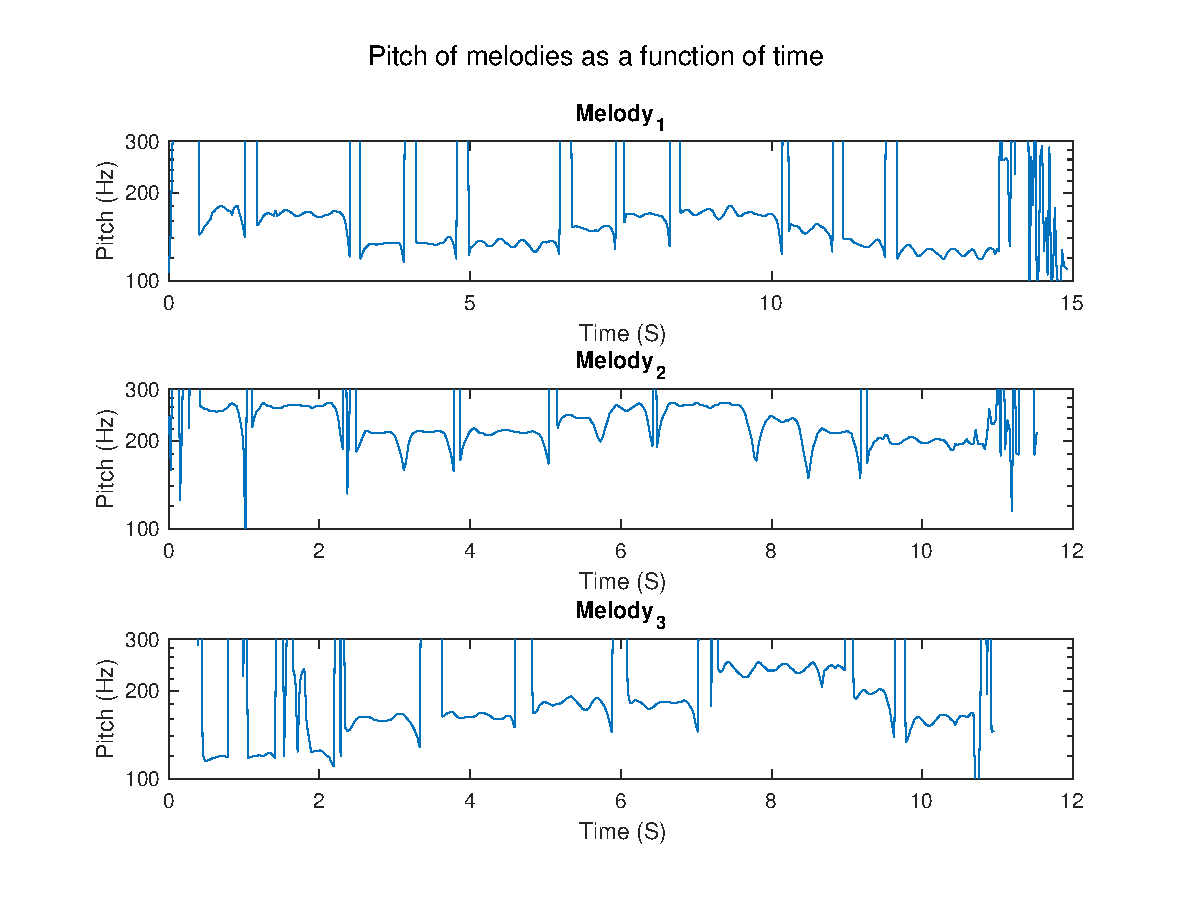
\includegraphics[width=\maxwidth{56.196688409433015em}]{figure_0.eps}
\end{center}


\begin{matlabcode}

\end{matlabcode}


\matlabheadingthree{Let's now plot the per-sample intensity, note that the time is still the same as the above figure.}

\begin{par}
\hfill \break
\end{par}

\begin{matlabcode}

figure;
sgtitle('Intensity of melodies as a function of time');
subplot(3,1,1);
plot(t_1, frIseqT1(3,:));
xlabel('Time (S)');
ylabel('Intensity');
title('Melody_1')

subplot(3,1,2);
plot(t_2, frIseqT2(3,:));
xlabel('Time (S)');
ylabel('Intensity');
title('Melody_2')

subplot(3,1,3);
plot(t_3, frIseqT3(3,:));
xlabel('Time (S)');
ylabel('Intensity');
title('Melody_3')
\end{matlabcode}
\begin{center}
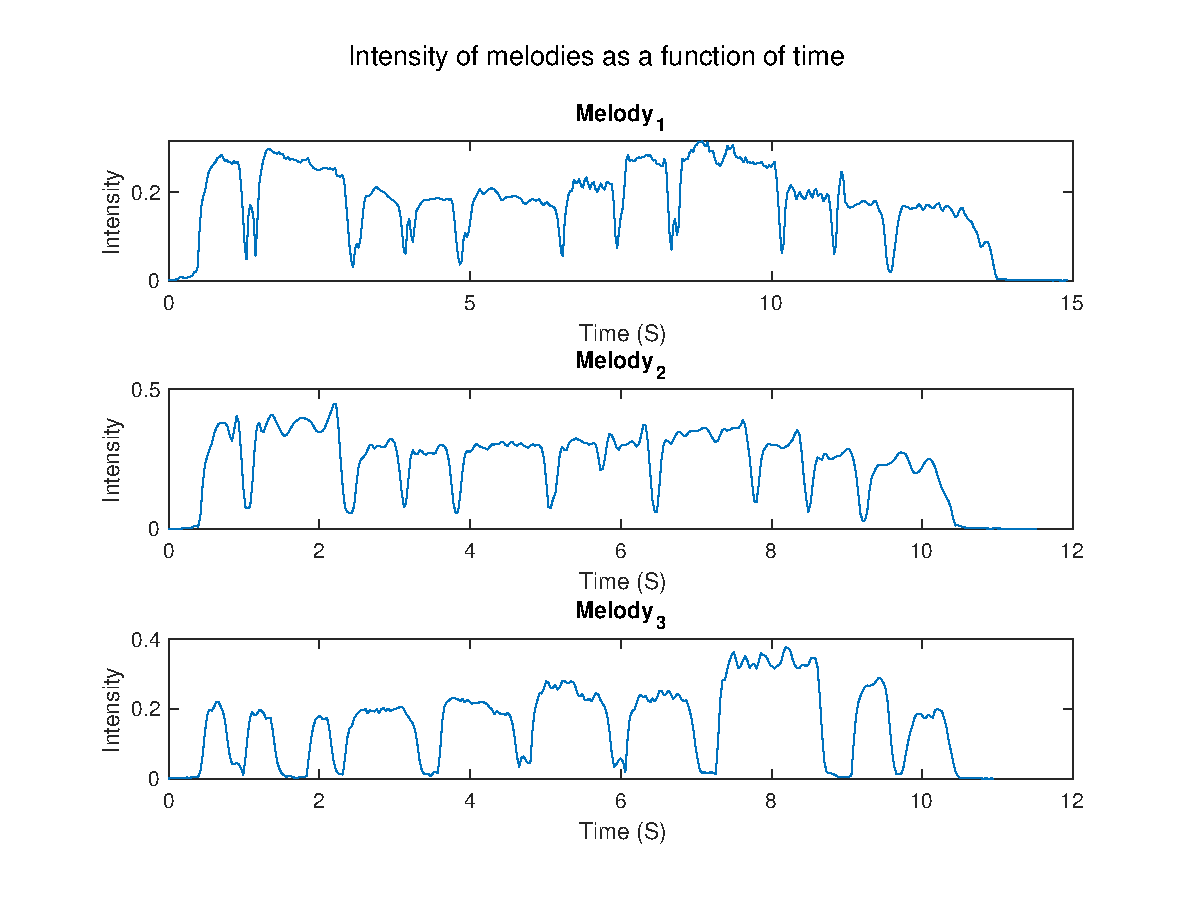
\includegraphics[width=\maxwidth{56.196688409433015em}]{figure_1.eps}
\end{center}
\begin{matlabcode}

\end{matlabcode}


\matlabheadingthree{Finally let's have look at the correlation, note that the time is still the same as the above figure. (Closer to one is better). This should tell who is the better singer.}

\begin{par}
\hfill \break
\end{par}

\begin{matlabcode}

figure;
sgtitle('Correlation between adjacent pitch periods as a function of time');
subplot(3,1,1);
plot(t_1, frIseqT1(2,:));
xlabel('Time (S)');
ylabel('Correlation (\rho)');
title('Melody_1')

subplot(3,1,2);
plot(t_2, frIseqT2(2,:));
xlabel('Time (S)');
ylabel('Correlation (\rho)');
title('Melody_2')

subplot(3,1,3);
plot(t_3, frIseqT3(2,:));
xlabel('Time (S)');
ylabel('Correlation (\rho)');
title('Melody_3')
\end{matlabcode}
\begin{center}
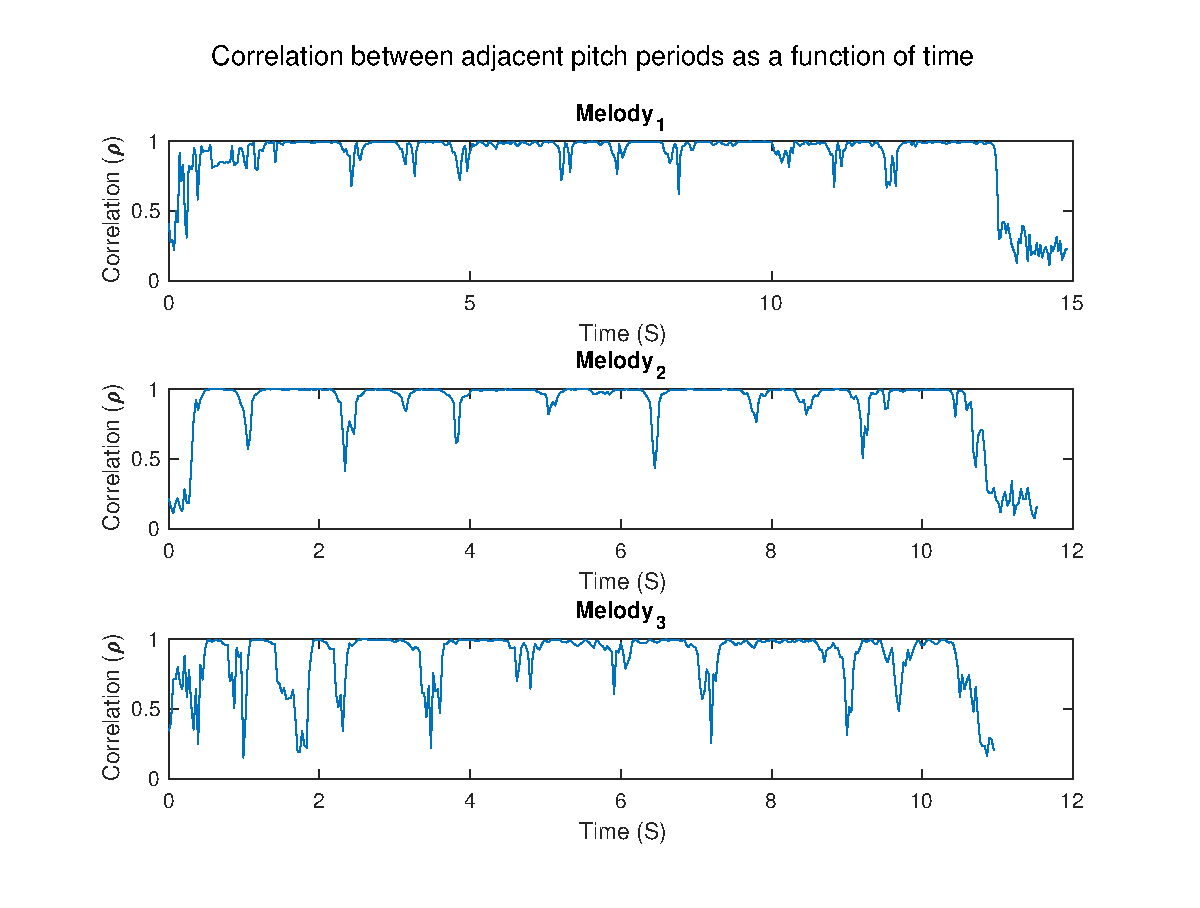
\includegraphics[width=\maxwidth{56.196688409433015em}]{figure_2.eps}
\end{center}


\matlabheading{Let's now use the postprocessing created in order to see if we can extraxt features that fit the hmm.}

\begin{matlabcode}
% ---- Uncomment the lines below if you want to verify that it works for
% ---- modifying the pitches.

%frIseqT1 = frIseqT1*3;
%frIseqT2 = frIseqT2*3;
%frIseqT3 = frIseqT3*3;
features_song_1 = Postprocess(frIseqT1);
features_song_2 = Postprocess(frIseqT2);
features_song_3 = Postprocess(frIseqT3);

\end{matlabcode}

\begin{par}
\begin{flushleft}
\href{https://se.mathworks.com/help/signal/ref/dtw.html}{\underline{https://se.mathworks.com/help/signal/ref/dtw.html}}
\end{flushleft}
\end{par}

\begin{matlabcode}
[d1, i11, i21] = dtw(features_song_1, features_song_2);
[d2, i12, i22] = dtw(features_song_2, features_song_3);
[d3, i13, i23] = dtw(features_song_1, features_song_3);
\end{matlabcode}


\begin{par}
\begin{flushleft}
We see above that the lowest value is actually yielded for melody 1 and 2, that being those that are from the same song. Further, we could try to plot the wrapped signals.
\end{flushleft}
\end{par}

\begin{matlabcode}
a1w = features_song_1(i11);
a2w = features_song_2(i21);

t = (0:lengthOfWindow:(numel(i11)-1)*lengthOfWindow);

duration = t(end)
\end{matlabcode}
\begin{matlaboutput}
duration = 19.5600
\end{matlaboutput}
\begin{matlabcode}
figure;
subplot(2,1,1)
plot(t,a1w)
title('Melody_1, Warped')
subplot(2,1,2)
plot(t,a2w)
title('Melody_2, Warped')
xlabel('Time (seconds)')
\end{matlabcode}
\begin{center}
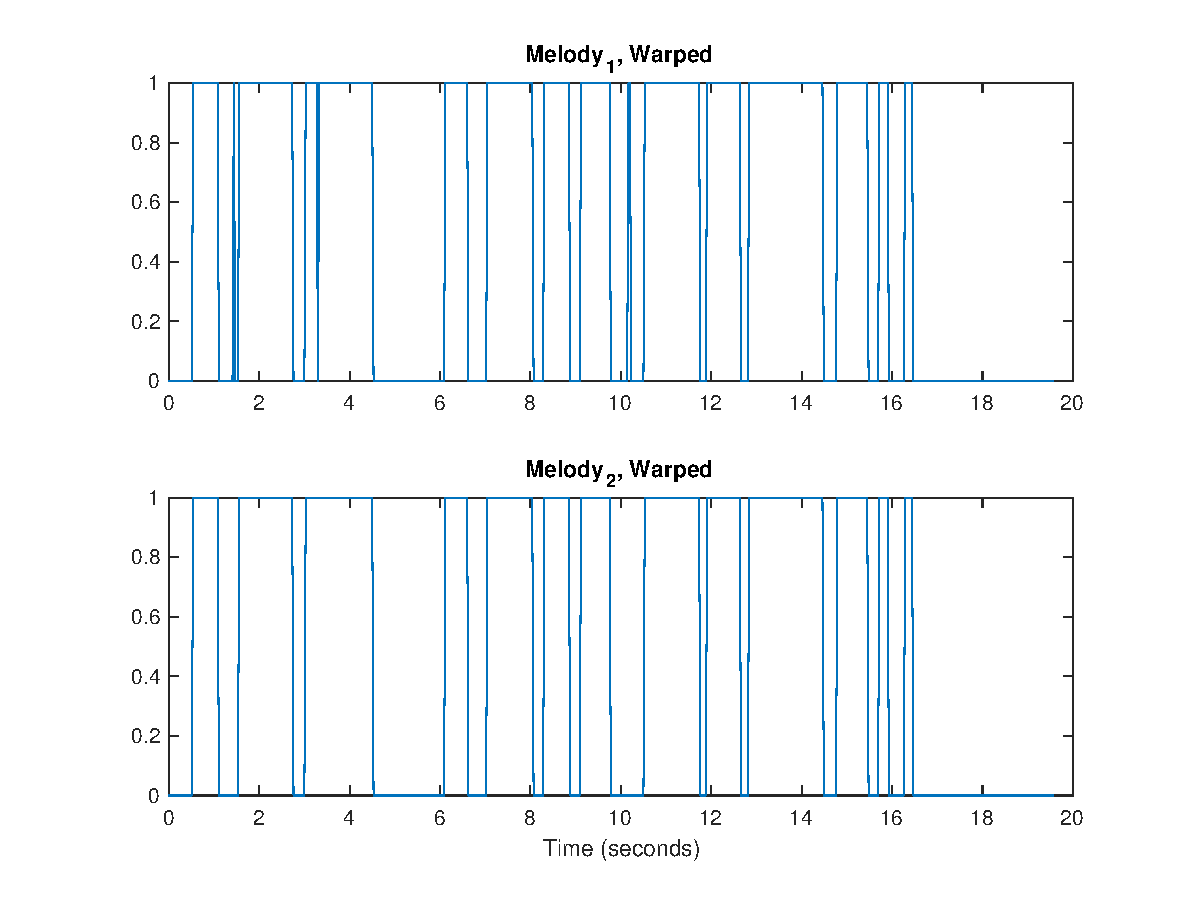
\includegraphics[width=\maxwidth{56.196688409433015em}]{figure_3.eps}
\end{center}


\begin{matlabcode}
a1w = features_song_1(i12);
a2w = features_song_3(i22);

t = (0:lengthOfWindow:(numel(i12)-1)*lengthOfWindow);

duration = t(end)
\end{matlabcode}
\begin{matlaboutput}
duration = 15.1500
\end{matlaboutput}
\begin{matlabcode}
subplot(2,1,1)
plot(t,a1w)
title('Melody_1, Warped')
subplot(2,1,2)
plot(t,a2w)
title('Melody_3, Warped')
xlabel('Time (seconds)')
\end{matlabcode}
\begin{center}
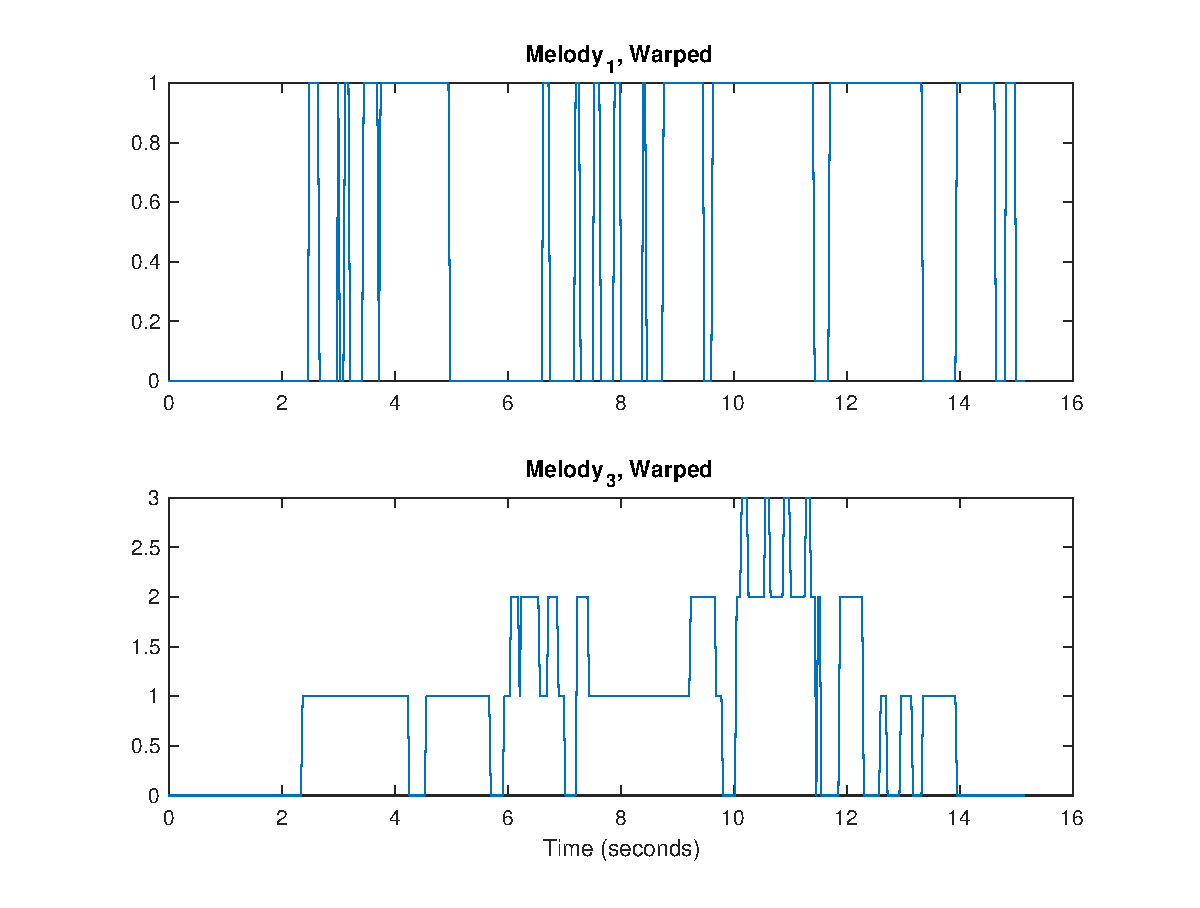
\includegraphics[width=\maxwidth{56.196688409433015em}]{figure_4.eps}
\end{center}


\begin{matlabcode}
a1w = features_song_1(i13);
a2w = features_song_3(i23);

t = (0:lengthOfWindow:(numel(i13)-1)*lengthOfWindow);

duration = t(end)
\end{matlabcode}
\begin{matlaboutput}
duration = 20.8800
\end{matlaboutput}
\begin{matlabcode}
subplot(2,1,1)
plot(t,a1w)
title('Melody_2, Warped')
subplot(2,1,2)
plot(t,a2w)
title('Melody_3, Warped')
xlabel('Time (seconds)')
\end{matlabcode}
\begin{center}
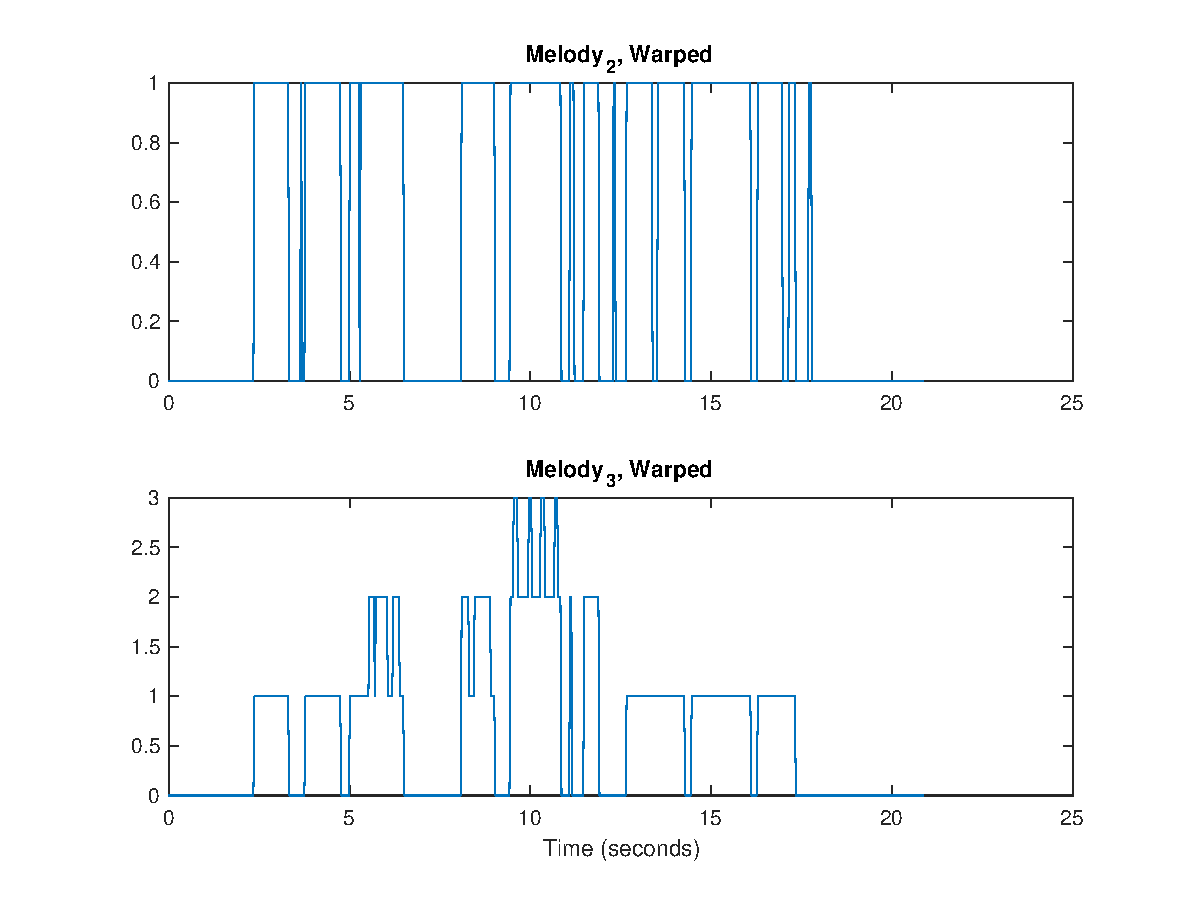
\includegraphics[width=\maxwidth{56.196688409433015em}]{figure_5.eps}
\end{center}


\begin{par}
\begin{flushleft}
\textbf{Finally, let's look at the distance between the signals that the dynamic time warping yielded.}
\end{flushleft}
\end{par}

\begin{matlabcode}
disp('---------x = 1.0 ---------')
\end{matlabcode}
\begin{matlaboutput}
---------x = 1.0 ---------
\end{matlaboutput}
\begin{matlabcode}
Distance_Melody1_and_2 = d1
\end{matlabcode}
\begin{matlaboutput}
Distance_Melody1_and_2 = 4
\end{matlaboutput}
\begin{matlabcode}
Distance_Melody1_and_3 = d2
\end{matlabcode}
\begin{matlaboutput}
Distance_Melody1_and_3 = 138
\end{matlaboutput}
\begin{matlabcode}
Distance_Melody2_and_3 = d3
\end{matlabcode}
\begin{matlaboutput}
Distance_Melody2_and_3 = 141
\end{matlaboutput}

\begin{par}
\begin{flushleft}
As we can clearly see, the distance between the signals of the first and second melody in lower than that of melody 1 and 3 and significantly lower than that of melody 2 and 3. Further, by visual inspection of the graphs above, it is clear that melody 1 \& 2 are more similair in shape than the others.
\end{flushleft}
\end{par}


\vspace{1em}
\matlabheadingtwo{Conclusion}

\begin{par}
\begin{flushleft}
By taking the logarithmic value of the frequency and intensity but leaving the relation values alone, we can calculate the mean and variance of the three features. By visualizing the data as a normal-distribution, we assume that we can use the mean and variance to identify noise and silent segments. This is done by marking values of frequency that falls outside of the interval$[\overline{frequency} -std(frequency),\overline{frequency} +std(frequency)]$ as noise, since these don't match the more common values and are thus regerded as outliers. Further, we mark the relationship values that falls below the mean as outliers (noise) and the same for intensity. As a stronger relation is better, we want to keep those values. As mentioned in the assignment, the model should not be sensitive to increased loadness (intensity), therefore we chose not to set an upper bound for outliers there.
\end{flushleft}
\end{par}


\vspace{1em}
\begin{par}
\begin{flushleft}
There are a few properties defined in the assignment that the feature extractor must have
\end{flushleft}
\end{par}

\begin{enumerate}
\setlength{\itemsep}{-1ex}
   \item{\begin{flushleft} The possibility to distinguish between diffrent melodier. - This is fulfilled as shown by warped melodies above. \end{flushleft}}
   \item{\begin{flushleft} Should allow to distinguish between note sequences with the same pitch track, but where note or pause durations differ. - This can be seen in how the time warped plots if melody\_1 and melody\_2 is very similair.  \end{flushleft}}
   \item{\begin{flushleft} The features are created by utalizing the \href{https://en.wikipedia.org/wiki/Twelfth_root_of_two}{Twelfth root of two}, which looks at the quotient between the base frequency (f\_0) and any other frequency at time t (f\_t) $12*log_2 (\frac{f_t }{f_0 })$ so any scalar transformation wont have effect. \end{flushleft}}
   \item{\begin{flushleft} Noises are filtered out with a hueristic that identifies outliers in the data and sets all those datapoints to 0, as the chosen feature output is discrete to out HMM. \end{flushleft}}
\end{enumerate}


\matlabheadingtwo{Robustness}

\begin{par}
\begin{flushleft}
To verify that the model (3) above, let us look at some transformations, where we multiply all values in melody\_1's vector with a value x.
\end{flushleft}
\end{par}

\matlabtitle{x = 0.5}

\begin{matlabcode}
features_song_1 = Postprocess(frIseqT1*0.5);
features_song_2 = Postprocess(frIseqT2);
features_song_3 = Postprocess(frIseqT3);

[d1, i11, i21] = dtw(features_song_1, features_song_2);
[d2, i12, i22] = dtw(features_song_2, features_song_3);
[d3, i13, i23] = dtw(features_song_1, features_song_3);
disp('---------x = 0.5---------')
\end{matlabcode}
\begin{matlaboutput}
---------x = 0.5---------
\end{matlaboutput}
\begin{matlabcode}
Distance_Melody1_and_2 = d1
\end{matlabcode}
\begin{matlaboutput}
Distance_Melody1_and_2 = 44
\end{matlaboutput}
\begin{matlabcode}
Distance_Melody1_and_3 = d2
\end{matlabcode}
\begin{matlaboutput}
Distance_Melody1_and_3 = 138
\end{matlaboutput}
\begin{matlabcode}
Distance_Melody2_and_3 = d3
\end{matlabcode}
\begin{matlaboutput}
Distance_Melody2_and_3 = 107
\end{matlaboutput}


\matlabtitle{x = 2 (one octave jump)}

\begin{matlabcode}
features_song_1 = Postprocess(frIseqT1*2);
features_song_2 = Postprocess(frIseqT2);
features_song_3 = Postprocess(frIseqT3);

[d1, i11, i21] = dtw(features_song_1, features_song_2);
[d2, i12, i22] = dtw(features_song_2, features_song_3);
[d3, i13, i23] = dtw(features_song_1, features_song_3);
disp('---------x = 2.0---------')
\end{matlabcode}
\begin{matlaboutput}
---------x = 2.0---------
\end{matlaboutput}
\begin{matlabcode}
Distance_Melody1_and_2 = d1
\end{matlabcode}
\begin{matlaboutput}
Distance_Melody1_and_2 = 1
\end{matlaboutput}
\begin{matlabcode}
Distance_Melody1_and_3 = d2
\end{matlabcode}
\begin{matlaboutput}
Distance_Melody1_and_3 = 138
\end{matlaboutput}
\begin{matlabcode}
Distance_Melody2_and_3 = d3
\end{matlabcode}
\begin{matlaboutput}
Distance_Melody2_and_3 = 130
\end{matlaboutput}


\matlabtitle{x = 2.5}

\begin{matlabcode}
features_song_1 = Postprocess(frIseqT1*2.5);
features_song_2 = Postprocess(frIseqT2);
features_song_3 = Postprocess(frIseqT3);

[d1, i11, i21] = dtw(features_song_1, features_song_2);
[d2, i12, i22] = dtw(features_song_2, features_song_3);
[d3, i13, i23] = dtw(features_song_1, features_song_3);
disp('---------x = 2.5---------')
\end{matlabcode}
\begin{matlaboutput}
---------x = 2.5---------
\end{matlaboutput}
\begin{matlabcode}
Distance_Melody1_and_2 = d1
\end{matlabcode}
\begin{matlaboutput}
Distance_Melody1_and_2 = 8
\end{matlaboutput}
\begin{matlabcode}
Distance_Melody1_and_3 = d2
\end{matlabcode}
\begin{matlaboutput}
Distance_Melody1_and_3 = 138
\end{matlaboutput}
\begin{matlabcode}
Distance_Melody2_and_3 = d3
\end{matlabcode}
\begin{matlaboutput}
Distance_Melody2_and_3 = 125
\end{matlaboutput}

\end{document}
